% !TeX spellcheck = cs_CZ

\chapter{Programátorská část}

Cíl pro letní semestr byl přenést simulaci do 3D a také vylepšit uživatelské rozhraní se kterým sem nebyl moc spokojený. Drtivá většina práce je tedy ve třídách spojených s \texttt{ImGuiViewer} neboť to je momentálně hlavní grafický výstup programu.
Níže jsou uvedeny jednotlivé věci, které prošly změnami a podrobněji se jim věnují další části této kapitoly. Pár věcí je ze seznamu rozšíření ze zimní dokumentace, ale i zde se nestihlo vše co by stálo za to implementovat. Takže na konci této kapitoly je seznam budoucích rozšíření/oprav.

\begin{enumerate}
	\item Předělána matematická knihovna a nově jsou podporovány generické 2D,3D,4D vektory a také 4D matice.
	\item Vytvořena kamera(třída \texttt{Camera}), která nahradila třídu \texttt{OMSAR}. Kamera slouží k orientaci a pohybu v prostoru, k čemuž využívá především matic.
	\item Knihovna \textbf{GLEW} nahrazena knihovnou \textbf{GLAD}
	\item Byla implementována podpora fyzikálních jednotek. Takže každá třída, která má přístup k datům si může zjistit v jakých jsou jednotkách a nemusí se spoléhat na konvence v komentářích.
	\item Reorganizace \texttt{ImGuiViewer}, kdy jeho podtřídy byly rozděleny na vykreslování uživatelského rozhraní a simulace.
	\item Kompletní přepsání kódu s uživatelským rozhraním.
	\item Vykreslování simulace je nyní plně ve 3D díky podpoře kamery včetně pár nových grafických prvků.
\end{enumerate}

\section{Matematická knihovna}
Návrh ze zimního semestru mi nepřišel moc šťastný, protože měl pevně zafixovaný datový typ na \texttt{double}. Což je sice dostačující pro samotnou simulaci, ale \textbf{OpenGL} má radši \texttt{float} a \textbf{ImGui} využívá pro kreslení UI \texttt{float} a \texttt{int}. Což si v důsledku vyžádalo zbytečné přetypovávání. Nová knihovna nabízí generické vektory, takže lze jednoduše použít \texttt{Vec3<double>} pro pozice simulovaných objektů, \texttt{Vec3<float>} pro potřeby OpenGL renderování. Nové generické matice využívá hlavně kamera při změně souřadnicových systémů při renderování scény.
Rychlý úvod do vektorů a matic pro potřeby 3D grafiky nabízí \cite{ostatniMatice}. Knihovna také rovnou obsahuje funkce pro perspektivní, ortogonální projekci, posunutí, otočení a škálování. Jejich implementace čerpá z \cite{projMatice,rotMatice,ostatniMatice}, kde jsou jejich vzorce intuitivně odvozeny, projekční matice jsou ještě upraveny pro potřebu OpenGL, což je popsáno v sekci \ref{par:depthBuffer}.


\section{Kamera}
Ve 2D stačilo pro globální pozici kamery definovat posunutí a škálování neboť byla kamera zafixována pro pohled ze shora bez možnosti rotace. Ve 3D je to vyřešené pomocí matic. 

Kamera je reprezentována abstraktní třídou \texttt{Camera}. Její orientace je dána pozicí kamery, sledovaného cíle a vektorem, který ukazuje vzhůru. Z toho je pomocí metody \texttt{LookAt()}, která má předchozí 3 argumenty,  postavena \textit{view} matice, která převádí objekty z globálních souřadnic(\textit{world space}) do souřadnic kamery(\textit{view space}). Dále je zde projekční matice, která převádí z \textit{view space} do normalizovaných souřadnic (\textit{clip space}), po vydělení čtvrtou souřadnicí $ w $ mají viditelné objekty souřadnice \textit{x, y, z} v rozsahu $ -1.0,1.0 $. S konvencí \textit{+x} vpravo,  \textit{+y} nahoru a \textit{-z} do obrazovky.
Jak je uvedeno v sekci \ref{par:depthBuffer} tak je lepší  \textit{z} přemapovat do $ \pm 1.0,0.0$ . Souřadné systémy nenáročně vysvětluje \cite{coords}.

\subsection{LookAt}
\label{sec:odvozKamery}
Metoda má prototyp \lstinline|LookAt(Vec3d poziceKamery, Vec3d poziceCile, Vec3d upVec)|, můžeme tedy ještě rovnou zavést \lstinline|smerKamery| jako \lstinline|poziceCile-poziceKamery|.

Předchozí sekce nám říká, že po transformaci \textit{view} a projekční maticí by směr kamery měl být $ (0,0,-1) $, směr vzhůru $ (0,1,0) $ a její pozice $ (0,0,0) $.  První dva vektory totiž perspektivní ani pravoúhlá projekce nemění, projekční matice ale definují $ near, far planes  $, které jsou dány relativně vůči pozici kamery a definují rozsah viditelné hloubky. Proto je pozice v počátku.Ještě dodefinujme \lstinline|rightVec| jako vektorový součin \lstinline|smerKamery| a \lstinline|upVec|, tedy vektor ukazující napravo od kamery. Poté ještě přepočítáme \lstinline|upVec| jako vektorový součin \lstinline|rightVec| a \lstinline|smerKamey|. Tím dostaneme 3 ortogonální, po znormalizování ortonormální, vektory.

Hledanou \textit{view} matici můžeme sestavit ve dvou krocích ( Stejně je to popsáno v \cite{lookAt}, ale orientace kamery není podle mě moc zdůvodněna), nejdříve je potřeba správně přesunout pozici kamery do počátku. To lze udělat následující maticí translace $ T $ ( $ T\times poziceKamery $ při rozšíření o $ poziceKamery.w=1 $ opravdu dává počátek)
\begin{align}
T=
\begin{pmatrix}
0 & 0 & 0 & -poziceKamery.x\\
0 & 0 & 0 & -poziceKamery.y\\
0 & 0 & 0 & -poziceKamery.z\\
0 & 0 & 0 & 1
\end{pmatrix}
\end{align}
Nyní potřebujeme ještě kameru natočit správným směrem. K tomu lze použít lineární algebru, můžeme si uvědomit, že otočení v tomto případě znamená změnu báze $ B_1 = \left\lbrace \texttt{rightVec},\texttt{upVec},\texttt{smerKamery}\right\rbrace $ na bázi 
$ B_2 = \left\lbrace (1,0,0),\texttt(0,1,0),\texttt(0,0,-1)\right\rbrace $.
Jednodušší je vyjádřit matici přechodu o $ B_2 $ k $ B_1 $, protože to stačí dát bázi $ B_1 $ do sloupců matice a otočit znaménko u směru kamery neboť $ B_2 $ je skoro kanonická báze. Hledaná matice otočení $ O $ je pak její inverze, což je v tomto případě pouze transpozice, protože je ortonormální. Výsledná matice $ O $ po rozšíření na $ 4\times4 $ je uvedena v \ref{eq:rot}. 
\begin{align}
\label{eq:rot}
O=
\begin{pmatrix}
rightVec.x & rightVec.y & rightVec.z & 0\\
upVec.x & upVec.y & upVec.z & 0\\
-smerKamery.x & -smerKamery.y & -smerKamery.z & 0\\
0 & 0 & 0 & 1
\end{pmatrix}
\end{align}
Hledaná $ view $ matice je pak pouze $ view=O\times T $.Výchozí implementace v \texttt{Camera.cpp} pracuje s otočeným směrem kamery, proto tam není opačné znaménko a také jsou obě matice už vynásobené.

\subsection{Ovládání kamery}

Je implementováno pomocí ovládáním myší, kdy táhnutím myš otáčí myšlenou jednotkovou koulí umístěnou uprostřed obrazovky, tento pohyb se přenáší na otáčení kamery kolem svého cíle.
Pro výpočet stačí myšlenku otočit a představit si, že myš se pohybuje po statické kouli, pak k výpočtu je pouze potřeba její počáteční a koncová pozice. Tyto pozice se převedou na vektory ze středu koule do obou bodů. Cosinus úhlu mezi oběma vektory je skalární součin(neboť mají délku 1) a vektorový součin dává osu rotace. Pak můžeme použít matici rotace okolo dané osy a tu aplikovat na kameru.
Pokud náhodou myš neleží na kouli (typicky rohy obrazovky), tak se její pozice definuje jako nejbližší bod na kouli.

Implementaci zajišťuje třída \texttt{CameraControls}. Navíc je k dispozici přibližování a oddalování kamery a také otáčení okolo své pozice nebo pohyb do stran.

\section{GLEW $ \rightarrow $ GLAD}

Toto není moc velká změna, ale koukal jsem že ji používá více projektu,tak jsem jí zkusil. Soubory si člověk vygeneruje přímo z oficiálních stránek\footnote{\url{http://glad.dav1d.de}}. Navíc je přímo vložená do projektu (jsou to jen dva soubory) a tím odpadla jedna ze dvou statických knihoven.

\section{Fyzikální jednotky}

Veškeré informace o simulovaných datech jsou uložený ve třídě \textit{SimData}. Ta ovšem neobsahovala žádnou informaci o tom v jakých jednotkách tyto data jsou a spoléhala se, že si to moduly nějak dohodnou mezi sebou. Což bylo jen formou komentářů v kódu.

Nyní byla vytvořena třída \textit{PhysUnits}, která obsahuje jednotky délky, času a hmotnosti a dovoluje mezi nimi převádět. \textit{SimData} pak používá instanci této třídy k implementaci různých funkcí pro převody hodnot v simulovaných datech. Navíc kdokoliv kdo dostane přístup k datům si může zjistit v jakých jsou jednotkách a podle toho se zařídit. Jednotlivé moduly se už nemusí domlouvat a každý si může pracovat ve vlastních jednotkách. 

\section{Reorganizace \texttt{ImGuiViewer}}
Tato třída je nyní jen jednoduchý wrapper okolo 4 tříd:
\begin{description}
	\item[OpenGLBackend] inicialuzuje OpenGL, GLFW, GLAD a vytváří okno pro kreslení.
	\item[ImGuiBackend] inicializuje knihovnu ImGui
	\item[GUIDrawer] Vykresluje uživatelské rozhraní.
	\item[SceneDrawer] Vykresluje 3D simulaci.
\end{description}
\section{Vykreslování simulace}
Vykreslování celé simulace organizuje třída \texttt{SceneDrawer}. Využívá k tomu následující třídy:
\begin{description}
 	\item[Camera, PerspectiveCamera, ScaledOrthoCamera] První třída je známá abstraktní třída z dřívejší sekce. Zbylé dvě jsou jejich konkrétní implementace s příslušnými projekcemi.
 	\texttt{SceneDrawer} se o obě třídy stará a dává je k dispozici ostatním částem programu.
 	
 	\item[CameraControls] ovládá kameru pomocí myši, které bylo také popsáno v dřívější sekci. Ovládání je vysvětleno v uživatelské příručce.
 	
 	\item[LineTrailsDrawer] Tato třída je už známá ze zimního semestru a zůstala skoro nezměněná až na 2D$ \rightarrow $3D pozice. Vykresluje historii pohybu simulovaných objektů.
 	
 	\item[SimDataDrawer] Se stará o vykreslování samotných objektů. Zde už bylo více změn, které jsou psány níže.
 	
 	\item[GridDrawer] Zcela nová třída, která vykresluje dynamickou 2D mřížku pro lepší orientaci v prostoru. Také nabízí projekci objektů na mříž ve formě třídy \texttt{PinHeads}. Její návrh je také vysvětlen níže.

\end{description}

\subsection{\texttt{SimDataDrawer}}
Nejdřív uděláme menší odbočku k OpenGL, protože vykreslování takových vzdáleností ve správném měřítku se neobešlo bez problémů.
\paragraph{Depth buffer}
\label{par:depthBuffer}
Je buffer, ve kterém je uložena hloubka objektů ve scéně. Při kreslení se tento buffer využívá k určení, které objekty mají být viditelné a které jsou schované za jinými. Většinou se jedná o 24bitový nebo 32bitový formát s fixed-point desetinnými čísly. Jejich rozsah může být dostatečný pro klasické aplikace, ale pro sluneční soustavu je nedostačující a dochází k \textit{z-fighting}, neboť program není schopný rozlišit hloubku mezi objekty a správně je vykreslit.
Hloubka není v bufferu uložena lineárně, ale větší rozsah je pro blízké objekty a zbylá část pro vzdálené, což je dobrá myšlenka neboť u vzdálených objektů stejně nebudou malé detaily vidět. Dobrý náhled toho jak jsou hodnoty uloženy a jak depth buffer funguje v OpenGL a co je \textit{z-fighting} je \cite{depthBuff}

Limitující faktor je nastavení rozsahu \textit{near,far plane} v projekční matici. Pro vyšší přesnost by tento rozsah měl být co nejmenší. Což ale znamená, že pro zachování přesnosti se do scény velmi vzdálené objekty prostě nevměstnají. Jednou z technik, kterou se dá docílit dostatečné přesnosti je, že se objekty rozdělí na blízké a vzdálené. Nejdříve se vykreslí vzdálené s $ near plane $ posunutým co nejdál a $ far plane $ za všemi objekty. Poté se buffer vymaže a vykreslí se blízké objekty s $ near plane $ blízko u kamery a $ far plane $ za blízkými objekty. Nevýhoda je, že se musí udržovat seznamy objektů dle vzdáleností, které se s pohybem kamery budou měnit. 

Tato technika by v našem případě fungovala, protože moc objektů nebudeme kreslit a není problém je tedy za běhu řadit. Lepší řešení je ale použít \textit{floating point} čísla, které dokáží uložit velké rozsahy hodnot. Zde, ale nastává problém pro OpenGL, protože Z je v rozsahu $ -1.0,\,+1.0 $, tak nám \textit{float} nepomůže, protože blízko $ \pm1.0 $ je exponent pevně daný a dostáváme přibližně stejné rozlišení jako \textit{fixed-point} čísla. Toto platí pro libovolné číslo kromě 0, čehož využívá následující technika (\textit{reversed depth buffer}) popsána v \cite{revBuff}. Místo rozsahu $ -1.0,\,+1.0 $ použijeme rozsah  $ 1.0,\,0.0  $. Blízko kamery bude přesnost zachována díky nelinearitě uložení a vzdálené objekty ji neztratí díky přesnosti \textit{float} čísel blízko 0. Podobnou metodu popisuje i \cite{logBuff}, ta zvyšuje přesnost použitím logaritmů a je o něco přesnější v případě 32bit formátu.

Rozhodl jsem se implementovat první techniku neboť nepotřebuje žádný zásah do shaderů. Ale na druhou stranu jsou potřeba rozšíření do OpenGL( \texttt{GL\_ARB\_clip\_control} nebo \texttt{GL\_NV\_depth\_buffer\_float}), popřípadě OpenGL 4.5. Ovšem i starší grafiky by s tím neměli mít problém, dle \cite{GLEXT} jsou obě rozšíření celkem rozšířená. Navíc jak popisuje článek \cite{revBuff}, tak je potřeba pozměnit projekční matice právě protože se Z mapuje jinak. Zde se s článkem trochu rozcházím, protože používám jinou projekční matici než je tam uvedena. Detaily změn jsou ve zdrojových kódech. Výsledek je ovšem stejný a k srovnání přesností se dá použít interaktivní graf v článku. Je nutné přepnout formát na float a pak je vidět obrovský rozdíl mezi \textit{Standard} a \textit{Reversed}. Popřípadě je dobrá webová aplikace \cite{srovnaniBuffer}(napsána v WebGL), která ukazuje rozdíl mezi klasickým a logaritmickým depth bufferem. Pro větší vzdálenosti klasická verze naprosto selhává.

Díky této technice není problém nastavit fixně \textit{near plane} na 1 metr a \textit{far plane} na 100 světelných let $ \approx 10^{18} $ metrů bez jakýkoliv problémů.
Její implementace je dostatečně popsána v samotném článku \cite{revBuff}, ale bylo čerpáno také z \cite{implRevBuff}.

\paragraph{Limity floating-point čísel}
V minulé části jsme vyřešili přesnost použítím \textit{floating-point čísel}, ovšem i tato čísla mají limity. Konkrétně 32bitový \textit{float} má přesnost přibližně 7 platných číslic a 64bitový \textit{double} 15. Pokud tedy bude mít objekt souřadnice $ (1m,0,0) $ tak v okolí nám \textit{float/double} dává přesnost přibližně $ 0,1 \mu m / 1fm$, což naše simulace určitě nikdy nevyužije. Co se stane když náš objekt bude v okolí Pluta? Tedy souřadnice $ (7\times10^{12}m,0,0) $, pak nám \textit{float/double} dává přesnost $ 700km,7mm $. To už je mnohem horší, Pluto má poloměr přibližně 1000km, takže ho ani \textit{float} nedokáže přesně reprezentovat. Bohužel platí, že čím dál jsme od počátku souřadnic, tím to bude horší. Více nejen o přesnosti $ floating-point $ čísel nabízí tento blog \cite{floatBlog}. V našem případě bylo zvoleno řešení už v zimě a to použít 64bit $ double $, jeho přesnost je o něco méně než metr ve vzdálenosti jednoho světelného roku od počátku.

Nyní ale nastává problém, že OpenGL a grafické karty mají radši 32bitová čísla, takže jednoduché řešení, že počátek umístíme do středu soustavy(cca Slunce) nám v případě Pluta nevykreslí hezkou kulatou planetku, ale něco co má do toho hodně daleko. Řešení, které jsem zvolil je, že počátek pro renderování nebude ve středu soustavy, ale na pozici kamery. Tím cokoliv co je blízko kamery bude i blízko počátku. Toto je možné jednoduše díky tomu, že přesné pozice, včetně kamery, zajišťuje použití \textit{double}, před posláním dat na grafiku stačí od pozic objektů odečíst pozici kamery, výsledek lze pak celkem bezpečně přetypovat na \textit{float}. Při použití této techniky je ale v shaderech naopak potřeba ignorovat posunutí objektů vůči kameře pomocí \textit{view} matice, což se udělá jednoduše vynulováním 3. sloupce matice viz. odvození matice v sekci \ref{sec:odvozKamery}.

Tato technika je implementována pro všechny následující třídy, ale nepoužívá ji \texttt{LineTrailsDrawer}. Což je vidět při přiblížení např. k Plutu, že čára za pohybem různě přeskakuje. Tahle podobně by skákaly všechny vertexy Pluta a nevypadá to moc hezky.

\paragraph{\texttt{SimDataDrawer}}
Nyní už k samotnému kreslení, všechny simulované objekty mají také svůj poloměr a je možné je vykreslit jako barevné 3D koule, což se také přesně děje. Ke kreslení využívá třídu \texttt{Sphere}, která vytvoří kouli a potřebná data pro OpenGL. 

Ovšem oddálením tak abychom viděli přibližně celou soustavu, zjistíme, že kromě Slunce nic nevidíme. Proto třída nabízí i vykreslování objektů s poloměrem v souřadnicích obrazovky, čili, že každý objekt bude tak velký aby byl vidět bez ohledu na jeho skutečnou velikost. Uživatelské rozhraní pak nabízí přepínání mezi oběma režimy. Korekce probíhá na základě hloubky objektu na obrazovce, neboť pokud je objekt dvakrát dále, tak je dvakrát menší, proto stačí poloměr právě jeho hloubkou vynásobit a tím bude nový poloměr invariantní vůči jeho hloubce. Malý detail je jednoduché osvětlení objektů Sluncem.
\subsection{\texttt{GridDrawer}}
Pokud bychom kreslili pouze samotné objekty, tak díky velkým vzdálenost a 360° pohybu kamery může člověk snadno ztratit orientaci, proto byla vytvořena tato třída která kreslí 2D mříž v prostoru a poskytuje tak orientační bod. Veřejné rozhraní také dovoluje zvolit přesnou pozici, velikost a orientaci mříže. Navíc nabízí zapnutí/vypnutí projekce jednotlivých objektů na mříž a spojení projekce s původním objektem, tím je hned vidět, kde se objekty v prostoru nachází vzhledem k ostatním.

\paragraph{\texttt{Grid}} je třída, která se stará o samotná data mříže(jednotlivé čáry) pro OpenGL. Kreslení pak organizuje \texttt{GridDrawer} pomocí dvou instancí této třídy. Dvě instance - větší a menší - nám dovolují dynamickou změnu velikosti mříže. Takže bez ohledu na to jak daleko jsme od objektů, vždy vidíme mříž s dostatečným rozlišením ( které je zobrazeno v uživatelském rozhraní ). 

\footnote{Před přečtením tohoto odstavce doporučuji pro lepší pochopení nejdříve program pustit a podívat se na výsledný pohyb mříže.} Implementace by tedy měla zajistit, že pokud dostatečně oddálíme kameru, tak malé čtverečky se \textbf{skokově} změní na větší a objeví se ještě větší a naopak. To přesně umožňují tyto dvě instance - menší se zvětší na větší a větší se také zvětší. Pokud bude tato změna správně napsaná, tak si uživatel ani ničeho nevšimne. Pro obě kamery \texttt{PerspectiveCamera} a \texttt{ScaledOrthoCamera} platí, že když ji desetkrát oddálíme, tak toho vidíme desetkrát více, nebo-li objekty se desetkrát zmenší. Pokud je tedy větší mříž $ k $-větší než menší, tak je potřeba najít funkci $ f(d) $, kde $ d>0 $ je vzdálenost kamery. Pro kterou platí, že když se $ d $ zvětší $ k$-krát, tak se také $ f(d) $ zvětší $ k $-krát a zároveň je vždy na intervalu $ (x_i,kx_i) $ konstantní, kde $ x_i $ jsou dána níže. Druhá podmínka je zde proto, aby se mříž změnila skokově a uživatel měl pocit, že mříž je součástí světa. Taková funkce je například \ref{eq:gridFunc}, její hodnoty jsou vykresleny v grafu \ref{graf:cameraFunc} pro $ k=2;\,5 $
\begin{align}
\label{eq:gridFunc}
f(d) = k^{\llcorner\log_kd\lrcorner}
\end{align}

Kde "$ \llcorner\lrcorner $" je dolní celá část. Bez ní by se jednalo o identitu $ f(d)=d $. Toto zaokrouhlení zajistí konstantnost na intervalech pro $ (k^i,k^{i+1}) , i\in Z $. Pro úplnost tedy $ x_i=k^i $.
Tuto funkci tedy využívá \texttt{GridDrawer} k správnému nastavení velikostí obou mříží \texttt{Grid}. Také na základě toho kde se v konstatním intervalu kamera vrovna nachází \texttt{GridDrawer} zajistí správné obarvené obou mříží, čímž se docílí hladkého přechodu.
Stejně jako u \texttt{SimDataDrawer} se ze stejných důvodů pro pozici mříže používají relativní souřadnice vůči kameře, navíc je pozice upravena tak, aby byla mříž vždy ve středu obrazovky.
\begin{figure}[h]
	\caption{Graf funkce \ref{eq:gridFunc}}
	\label{graf:cameraFunc}
	\centering
	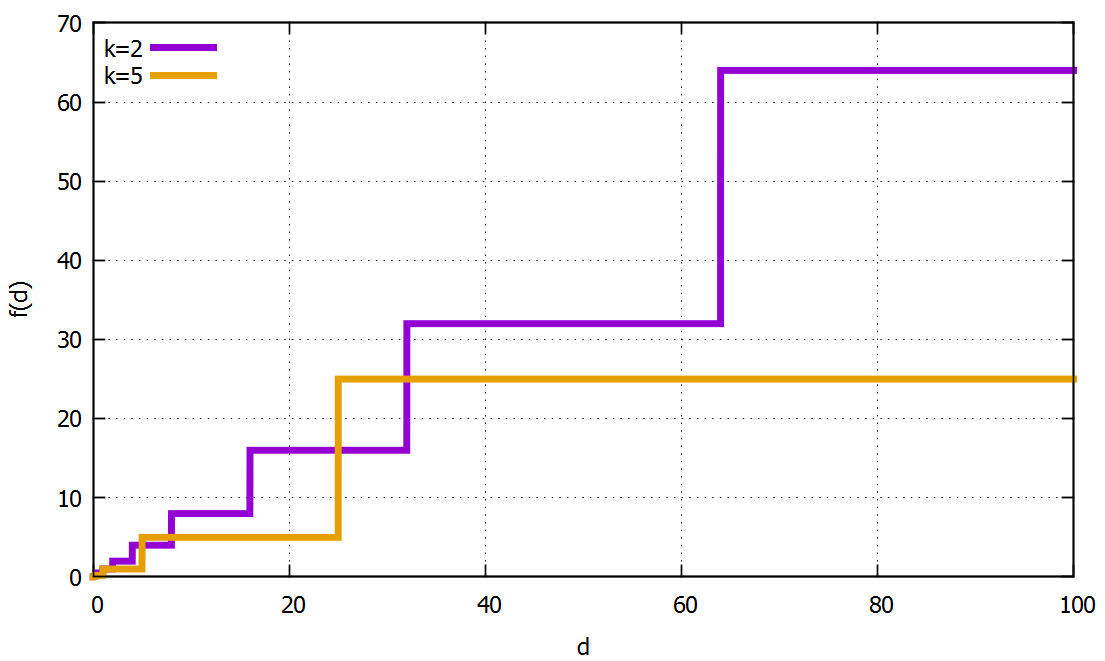
\includegraphics[width=\linewidth,keepaspectratio]{Figs/plotCameraFnc}\\
\end{figure}
\FloatBarrier
\paragraph{\texttt{PinHeads}}\footnote{Protože to spolu s vykreslením objektů jako koulí vypadá jako špendlíková hlavička zapíchnutá v mřížce.}je třída, která se stará o vykreslení projekcí objektů na mříž k čemuž jí stačí znát pozici všech těchto objektů a samotné mřížky, poté pro každý objekt vykreslí(pomocí \textit{geometry shader}ů OpenGL) projekci i spojení s objektem. Pro pozice také používá relativní souřadnice vůči kameře.


\section{Nové uživatelské rozhraní}
Uživatelské rozhraní bylo kompletně přepsáno. Jeho hlavní třídou je \texttt{GUIDrawer}, který vykresluje horní, spodní lištu a popřípadě všechna okna implementovaná v následujících třídách:
\begin{enumerate}	
	\item \texttt{UnitsProperties} - Seznam všech simulovaných objektů a jejich fyzikálních vlastností.
	\item \texttt{Graphs} - Dovoluje vytvářet grafy různých fyzikálních veličin - vzdálenost, rychlost, energie objektů.
	\item \texttt{ObjectContextMenu} - Najetím/Kliknutím myší na objekty se objeví toto okno, které ukazuje jméno objektu a dovoluje objekt sledovat nebo se k němu přiblížit.
	\item \texttt{VisualPreferences} - Okno s různými nastaveními grafiky a kamery.
	\item \texttt{SimProperties} - Zobrazuje detaily o průběhu simulace.
\end{enumerate}
Detaily implementace těchto tříd by měly být jasné při pohledu do zdrojových kódu, které hlavně využívají knihovnu \textbf{ImGui}. 
\section{Vylepšení a opravy}
Stejně jako v zimě jsem si průběhu práce na programu vedl v souboru plán toho, na čem budu pracovat, časem
se tam objevily různé nápady, které se do programu hlavně z časových důvodů nevešly, proto
je zmíním alespoň zde:
\begin{description}
	\item \textbf{Zaznamenávání a přehrávání simulace} \\
	S tímto tématem jsem od zimy vůbec nepohnul až na pár oprav aby zůstalo funkční. Ale myslím si, že je užitečné a stálo by za to ho dodělat. Pořád platí, že by se mělo ukládat v \texttt{simMethod}, že lineární interpolace je nic moc a že uživatel to může také celé rozbít změnou rychlosti simulace pomocí tlačítek, které jsou zapnutá. S tím souvisí další bod.
	\item \textbf{\texttt{Traits} pro moduly}
	Momentálně může každý modul měnit vlastnosti simulace, případně přidávat/mazat objekty za chodu bez ohledu na to, zda to ostatní moduly zvládnou, jakože momentálně spíš nezvládnou. Můj návrh by byl pro každý modul definovat specializaci třídy \texttt{SimTraits}, která by v sobě držela podmínky, které modul vyžaduje. Pak by mělo stačit aby konstruktor \texttt{Simulation} používal šablony (\textit{templates}) a ověřil při kompilaci zda jsou jednotlivé moduly navzájem kompatibilní.
	Navíc by to mohlo vést k tomu, že by třída \texttt{Unit} mohla obsahovat různé proměnné(nebo pointer na nějaké \texttt
	{ExtraInfo}) právě dle požadavků modulů místo fixní barvy a poloměru, které se simulací nesouvisí.
	\item \textbf{\texttt{LineTrails}} by měla používat relativní souřadnice. Ale bylo nutné držet pozice v \textit{double} a kopírovat relativní pozice do vertex bufferu každý frame, což je nic moc. Proto by bylo lepší zavést něco jako strom souřadnic - třeba \textit{octree}, kde každý blok by si počítal souřadnice vzhledem ke svému počátku. Pokud by spodní bloky s objekty byly dostatečně malé, tak by na ně stačil \textit{float}. Ale to za přesnější čáry za objekty nestojí.
	\item \textbf{Lepší ovládání kamery} Kamera se momentálně ovládá pouze myší, chtělo by to přidat ovládání i pomocí klávesnice. Také by stálo za to přidat možnost zafixování pozice kamery relativně k danému objektu. 
	\item \textbf{Vylepšit grafy} Nyní je to taková verze 0.8, kdy většina věcí funguje, ale je potřeba doladit vizuální mouchy a ovládání je takové nic moc = neintuitivní. Například by bylo lepší použít stejný algoritmus pro mřížku jako \texttt{GridDrawer} a nějaký ucelený systém jednotek.
	\item \textbf{Keplerovy zákony}
	Nebylo by špatné vidět implementaci Keplerových zákonů a případně srovnat výstup s numerickými metodami.
	\item \textbf{Launch window} S trochou snahy by nemělo být těžké aby aplikace po spuštění vytvořila malé okno s nastavením simulace a poté ji spustila, bylo by to hezčí než používat příkazovou řádku (ale ta by také zůstala). Navíc vše pro tvorbu okna už je implementované v \texttt{ImGuiViewer}.
	\item \textbf{Hezčí vzhled} je spíš můj osobní a hodně vzdálený cíl, aby Sluneční soustava vypadala realisticky. Což by obnášelo použít textury pro planety, přidat simulaci atmosféry \footnote{ http://www-evasion.imag.fr/people/Eric.Bruneton/  - \textit{Atmosphere} - Moc tomu ještě nerozumím, ale vypadá to hezky.} a také přidat třeba skybox s hvězdami nebo prstence kolem planet a hezčí osvětlení.
\end{description}


